%%%%%%%%%%  TEMPLATE LAST EDITED BY PRADIPTA GHOSH on 18/01/2020 %%%%%%%%%%%%%%%%%%%%
%
%  PYD411 MID-TERM REPORT  --  Phase-field modelling of cell crawling
%
%  COMPILE WITH pdflatex (twice).
%
%  SUBMITTED PDF NAME (do not miss the two underscores)
%      THEME_FULL-ENTRY-NUMBER_2601PYD411_MR.pdf
%
%%%%%%%%%%%%%%%%%%%%%%%%%%%%%%%%%%%%%%%%%%%%%%%%%%%%%%%%%%%%%%%%%%%%%%%%%%%%
\documentclass[11pt]{article}
\voffset=-2.8cm
\hoffset=-1.6cm
\textwidth=14.5cm
\textheight=24.5cm
\usepackage{amsmath}
\usepackage{amsfonts}
\usepackage{amssymb}
\usepackage{epsfig}
\usepackage{hyperref}
\usepackage[caption=false]{subfig}
\usepackage{soul,xcolor}
\usepackage{float}

\setlength{\parskip}{2pt}
\setlength{\abovedisplayskip}{4pt}
\setlength{\belowdisplayskip}{4pt}
\setlength{\floatsep}{8pt}
\setlength{\textfloatsep}{8pt}
\setlength{\intextsep}{8pt}
\makeatletter
\renewcommand{\section}{\@startsection{section}{1}{\z@}%
  {-1.2ex plus -0.2ex}{0.6ex}{\normalfont\large\bfseries}}
\makeatother

%%%%%%%%%%%%%%%%%%%%%%%%%%%%%%%%%%%%%%%%%%%%%%%%%%%%%%%%%%%%%%%%%%%
\begin{document}
%%%%%%%%%%%%%%%%%%%%%%%%%%%%%%%%%%%%%%%%%%%%%%%%%%%%%%%%%%%%%%%%%%%
\thispagestyle{empty}
\begin{center}
 
\includegraphics[height=2.4cm,angle=0]{Logo-IITD.jpg}\\[2pt]
\textbf{Dept of Physics, IIT Delhi}\\[4pt]
\textbf{Course Code : PYD411}\\
\textbf{Academic Year : 2026 - 2027,\, Semester - I}\\
\textbf{Mid-term Progress Report}\\[6pt]
\textbf{\LARGE{Phase-Field Modelling of Crawling Cells}}\\[2pt]
\textbf{\large{Towards a Tractable Two-Dimensional Model}}\\[8pt]
\textbf{\large{Siddharth Kumar (2023PH10741)}}\\
\textbf{\large{Soumik Roy (2023PH10756)}}\\[4pt]
\textbf{\large{Adviser: Prof.\ Sujin B.\ Babu}}
\end{center}

\vspace{6pt}
\noindent
\textbf{Abstract}:
We implement a continuum phase-field model of eukaryotic cell crawling,
coupling a cell field $\phi$ to an actin polarization $\mathbf{P}$, following
Tjhung \textit{et al.}~\cite{Tjhung:2015} and the effective-adhesion picture of
Leoni and Sens~\cite{Leoni:2017}. The model is built in four stages so that
each physical ingredient can be isolated. A baseline with vanishing fluid
velocity translates a cell but cannot deform it and loses $4.5\%$ of its area.
Confining treadmilling to a wall layer produces a leading protrusion and a
transition in the treadmilling rate. The complete plane model, with Stokes
flow, active stress and anchoring, recovers the non-motile actin aster and the
lamellipodial fan. Isolating ingredients shows that in this geometry the shape
is set almost entirely by anchoring-induced splay of $\mathbf{P}$; the flow
contributes about $2\%$. We therefore replace the elliptic Stokes solve by its
friction-dominated limit. The reduced model crawls steadily (travel $239.9$
in time $299$ at speed $0.801$), is about five times faster, agrees with the
full calculation to $0.2\%$ where they coincide, conserves volume rather than
projected area, and is local --- the property needed for many interacting cells.

\vspace{10pt}
\begin{flushleft}
Signature of the student 1: ................\\[6pt]
Signature of the student 2: ................
\end{flushleft}
\vspace*{-1.35cm}
\begin{flushright}
Signature of the adviser: ................
\end{flushright}

\vspace{4pt}
\pagestyle{plain}
\small
\setcounter{page}{1}
\setlength{\parskip}{1pt}
\setlength{\abovedisplayskip}{3pt}
\setlength{\belowdisplayskip}{3pt}
\setlength{\floatsep}{5pt}
\setlength{\textfloatsep}{5pt}
\setlength{\intextsep}{5pt}
%%%%%%%%%%%%%%%%%%%%%%%%%%%%%%%%%%%%%%%%%%%%%%%%%%%%%%%%%%%%
\section{Introduction and Motivation}
\label{sec:intro}

\noindent
Cell crawling on a substrate underlies wound healing, immune response and
metastasis. Mechanically it combines actin treadmilling at the front,
myosin-driven contraction at the rear, and focal adhesions that couple the
network to the substrate~\cite{Bray:2000}. Keratocyte fragments that lack the
nucleus still polarise and crawl~\cite{Verkhovsky:1999}, and motile shapes can
be predicted from a few mechanical parameters~\cite{Keren:2008}. This
motivates minimal physical models.

Tjhung, Tiribocchi, Marenduzzo and Cates~\cite{Tjhung:2015} treat a crawling
cell as a droplet of active polar fluid and, in three dimensions, obtain a
fried-egg aster, a keratocyte-like lamellipodium and a finger-like
pseudopod. Averaged over stochastic mechanosensitive linkers, substrate
adhesion reduces to an effective friction~\cite{Leoni:2017}, which is how it
enters depth-averaged continuum models~\cite{Ziebert:2013}. The long-term goal
of this project is many interacting cells. The Stokes solve of
Ref.~\cite{Tjhung:2015} is elliptic, hence expensive for one cell and
prohibitive for many. The mid-term work therefore implements the full model,
identifies which ingredients actually matter, and constructs a cheaper model
whose accuracy we can quantify (Table~\ref{tab:versions}).

\begin{center}
\begin{minipage}{\textwidth}
\centering
\begin{tabular}{|l|l|l|l|}
\hline
Ver. & Geometry & Force balance & Area \\
\hline
1 & plane, free space & $\mathbf{v}=0$ & drifts $4.5\%$ \\
\hline
2 & slice with a wall & screened in $z$ & fixed exactly \\
\hline
3 & plane & incompressible Stokes & fixed exactly \\
\hline
4 & plane & friction dominated & free, soft \\
\hline
\end{tabular}\\[3pt]
\refstepcounter{table}\label{tab:versions}
{\small Table~\thetable: Four stages of the model. Versions~2 and~3 are
complementary (side view vs.\ top view). Version~4 is the tractable model
for later multi-cell work.}
\end{minipage}
\end{center}

%%%%%%%%%%%%%%%%%%%%%%%%%%%%%%%%%%%%%%%%%%%%%%%%%%%%%%%%%%%%
\section{Computational Setup}
\label{sec:model}

\noindent
The cell is a diffuse field $\phi$ ($1$ inside, $0$ outside);
$\mathbf{P}$ is the coarse-grained actin polarization; $\mathbf{v}$ is the
cytoplasmic velocity. Following Ref.~\cite{Tjhung:2015},
\begin{eqnarray}\label{eq:F}
F=\int\!d^2r\,\Bigl\{
a\phi^{2}(\phi-1)^{2}
+\tfrac{\varepsilon^{2}}{2}|\nabla\phi|^{2}
-\tfrac{\alpha}{2}(2\phi-1)|\mathbf{P}|^{2}
&&\nonumber\\
+\tfrac{\alpha}{4}|\mathbf{P}|^{4}
+\tfrac{\kappa}{2}(\nabla\mathbf{P})^{2}
+\beta\,\mathbf{P}\cdot\nabla\phi\Bigr\}.
\end{eqnarray}
The first two terms generate interfacial tension. The $\alpha$ terms drive
$|\mathbf{P}|^{2}=2\phi-1$ inside the cell only. The Frank term aligns
neighbouring actin. Anchoring $\beta>0$ points $\mathbf{P}$ outward, normal
to the boundary, and is the controlling shape parameter. Transport is by
$\mathbf{u}=\mathbf{v}+w_{0}\mathbf{P}$, with $w_{0}$ the treadmilling
(polymerisation) speed:
\begin{equation}\label{eq:eom}
\partial_t\phi+\nabla\cdot(\phi\mathbf{u})
=-M\bigl[\mu_\phi-\Lambda g(\phi)\bigr],\qquad
\partial_t\mathbf{P}+(\mathbf{u}\cdot\nabla)\mathbf{P}
=-\boldsymbol{\Omega}\cdot\mathbf{P}+\chi\mathbf{D}\cdot\mathbf{P}
-\mathbf{h}/\Gamma,
\end{equation}
where $\mu_\phi=\delta F/\delta\phi$, $\mathbf{h}=\delta F/\delta\mathbf{P}$,
$g=\phi(1-\phi)$, and $\mathbf{D}$, $\boldsymbol{\Omega}$ are the strain-rate and
vorticity. At Reynolds number $\sim10^{-5}$ the force balance is Stokes. In a
top view the wall of Ref.~\cite{Tjhung:2015} becomes a depth-averaged friction
$-\xi\mathbf{v}$~\cite{Leoni:2017},
\begin{equation}\label{eq:stokes}
0=-\nabla p+\eta\nabla^{2}\mathbf{v}-\xi\mathbf{v}+\mathbf{f},\qquad
\nabla\cdot\mathbf{v}=0,
\end{equation}
with $\mathbf{f}=\nabla\cdot(\sigma^{\mathrm{act}}+\sigma^{\mathrm{el}})
-\phi\nabla\mu_\phi$ and
$\sigma^{\mathrm{act}}_{\alpha\beta}=-\zeta\phi P_\alpha P_\beta$
($\zeta<0$ contractile). Version~3 solves~(\ref{eq:stokes}) spectrally.
Version~4 uses $\eta/(\xi R^{2})\approx0.006$ for $R\approx13$: friction, not
viscosity, balances the active forces, leaving the local Darcy law
$\mathbf{v}=\mathbf{f}/\xi$.

Versions~2 and~3 enforce rigid area with a spatially uniform Lagrange
multiplier $\Lambda=\int\mu_\phi/\int g$~\cite{Rubinstein:1992}.
A real cell has roughly constant \textit{volume} $V_{0}\simeq hA$, so
spreading is allowed if paid for by thinning; Version~4 uses the soft law
$\Lambda=-k_{A}(A/A_{0}-1)$. Advection is written in conservative flux form
on a periodic grid and advanced by explicit Euler.

%%%%%%%%%%%%%%%%%%%%%%%%%%%%%%%%%%%%%%%%%%%%%%%%%%%%%%%%%%%%
\section{Results and discussion}
\label{sec:results}

\noindent
\textbf{Version 1.}
With $\mathbf{v}=\zeta=\beta=0$ a disc translates but cannot change shape
(uniform $\mathbf{P}$ gives uniform $\mathbf{u}$) and loses $4.5\%$ of its
area to non-conservative advection.

\textbf{Version 2: protrusion at the wall.}
The thin protrusion of Ref.~\cite{Tjhung:2015} is a near-substrate structure,
so we work in a vertical $(y,z)$ slice with
$w(z)=\frac{w_{0}}{2}\bigl[1-\tanh((z-\lambda)/w_\tau)\bigr]$
and the Brinkman closure
$(1-\ell_v^{2}\partial_z^{2})\mathbf{u}=w(z)\mathbf{P}$,
$\ell_v=\sqrt{\eta/\xi}$. Near-wall material runs out ahead of the body;
tension pulls it back; that competition \textit{is} the protrusion
(Fig.~\ref{fig:v2}a,b). At $w_{0}=0.3$ the cell stays a hemispherical
cap (contact length $44.0$, speed $0.050$); at $w_{0}=2.0$ it draws a thin
leading layer (contact $63.0$, speed $0.432$). Volume is conserved to
$10^{-16}$.

Sweeping $w_{0}$ (Fig.~\ref{fig:v2}c) shows the protrusion transition: the
contact length is nearly flat below $w_{0}\approx0.8$ and then rises
steeply, close to $M\varepsilon^{2}/\lambda\approx0.75$. The lamella length
and crawl speed rise in the same window.

\begin{figure}[H]
\centering
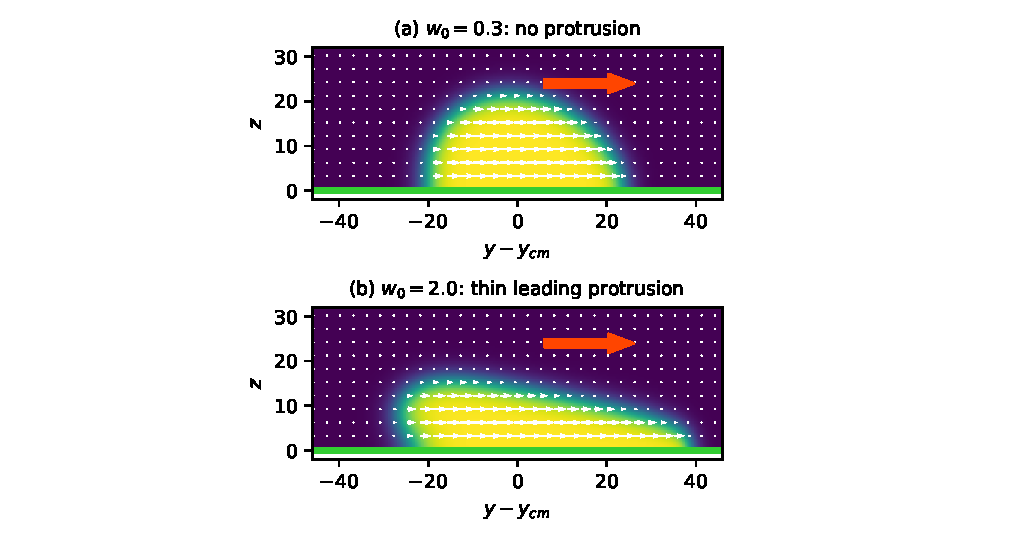
\includegraphics[width=13.2cm,height=4.15cm,keepaspectratio]{figures/fig_v2_shapes.pdf}\\[3pt]
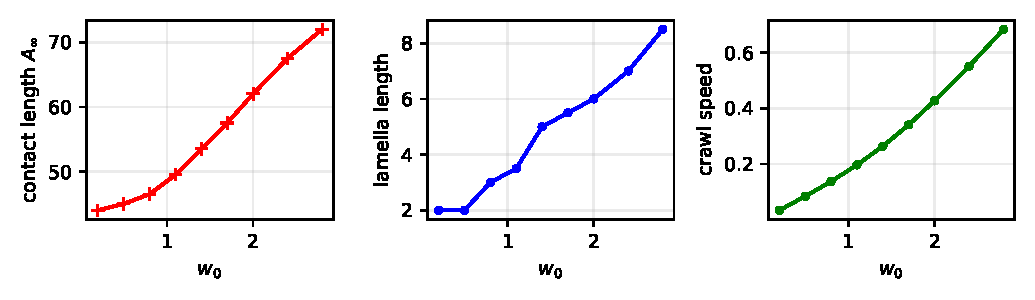
\includegraphics[width=13.2cm,height=2.55cm,keepaspectratio]{figures/fig_v2_transition.pdf}
\caption{Version~2. Top: vertical slice, wall at $z=0$ (green);
(a)~$w_{0}=0.3$, hemispherical cap; (b)~$w_{0}=2.0$, thin leading
protrusion. Arrows: $\mathbf{P}$. Volume error $10^{-16}$.
Bottom: contact length, lamella length and crawl speed versus $w_{0}$.}
\label{fig:v2}
\end{figure}

\textbf{Version 3: shapes in the plane.}
The catalogued shapes of Ref.~\cite{Tjhung:2015} are top views, so Version~3
solves the complete plane system. The passive limit is verified first: an
ellipse relaxes to a circle (aspect $1.689\to1.010$), the free energy
decreases, the flow dies and the volume error is exactly zero.

With activity (Fig.~\ref{fig:v3}, top), strong outward anchoring locks
$\mathbf{P}$ into a radial aster: $|\langle\mathbf{P}\rangle|=0$ and the
speed is zero to machine precision, the fried egg of
Ref.~\cite{Tjhung:2015} and of experiment~\cite{Yam:2007}. Moderate anchoring
gives a fan elongated \textit{across} the path (aspect $2.91$, speed
$0.843\approx w_{0}$), the keratocyte lamellipodium. Driving anchoring harder
gives a more extreme fan (aspect $4.35$). A plane pseudopod cannot form
(contractility only widens the cell) and the phagocytic cup is
three-dimensional; Version~2 already captures the vertical mechanism of the
former.

\begin{figure}[H]
\centering
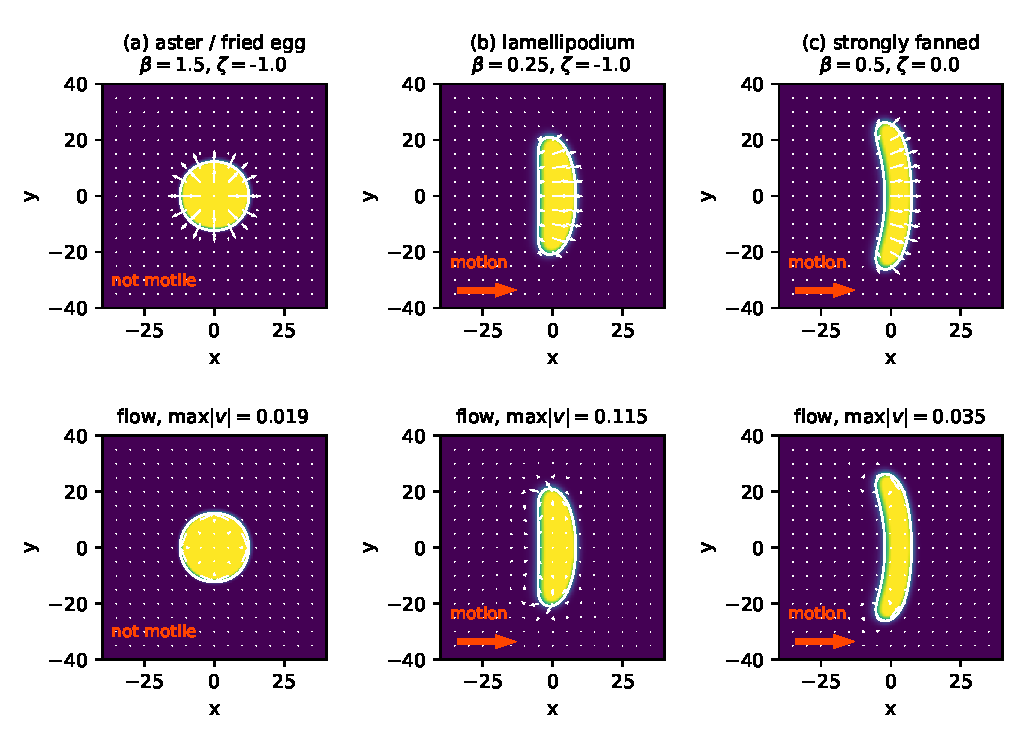
\includegraphics[width=13.2cm,height=5.4cm,keepaspectratio]{figures/fig_v3_morph.pdf}\\[3pt]
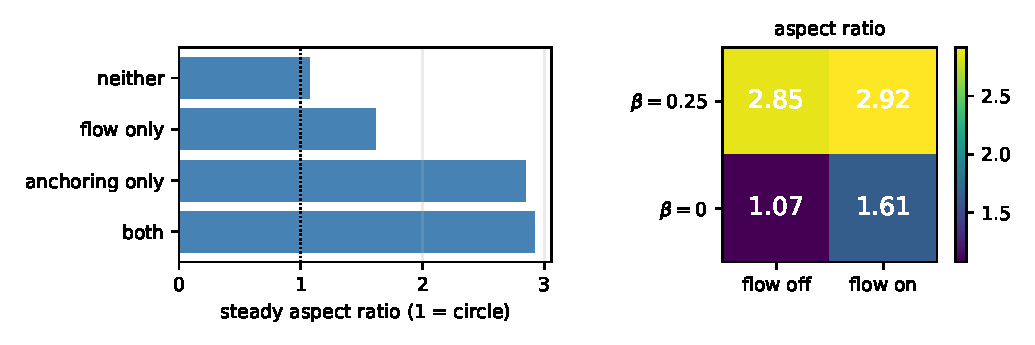
\includegraphics[width=13.2cm,height=2.7cm,keepaspectratio]{figures/fig_v3_decomp.pdf}
\caption{Version~3. Top: morphologies at $w_{0}=1$ --- $\phi$ and
$\mathbf{P}$ (upper row) and flow $\mathbf{v}$ (lower row).
(a)~Aster, not motile. (b)~Lamellipodial fan, aspect $2.91$, speed $0.843$.
(c)~Stronger fan, aspect $4.35$. Bottom: $2\times2$ of anchoring vs.\ flow;
anchoring alone $1.07\to2.85$, both together $2.92$ ($+2\%$).}
\label{fig:v3}
\end{figure}

A $2\times2$ control (Fig.~\ref{fig:v3}, bottom) isolates the two shape
mechanisms. Neither: translating disc, aspect $1.07$. Flow alone: $1.61$.
Anchoring alone: $2.85$. Both: $2.92$ ($\approx2\%$ above anchoring). Speed
is $0.80$--$0.85$ in every case, set by $w_{0}\langle\mathbf{P}\rangle$.
Sweeping $\xi$ over a $32$-fold range screens the flow as $1/\xi$, leaves the
speed almost unchanged ($0.829$--$0.845$), and saturates the aspect onto the
flow-free value $2.85$. The flat speed disagrees with the biphasic curve of
Ref.~\cite{Leoni:2017}: there propulsion is traction and requires
mechanosensitive bonds, which a constant $\xi$ cannot see.

\textbf{Version 4: a crawling cell without Stokes.}
The Darcy reduction is local and algebraic. Only the active part
$\mathbf{v}=-(\zeta/\xi)\nabla\cdot(\phi\mathbf{P}\mathbf{P})$ is kept
(vorticity and flow alignment change the shape by $<1\%$). Contractility is
recalibrated to $\zeta=-0.25$ (without pressure the same $\zeta$ is
$\sim10\times$ too strong).

Figure~\ref{fig:v4} is the main result. In the laboratory frame the cell
travels $239.9$ length units in time $299$ at a steady speed $0.801$: the
circular seed becomes a fan elongated across its path and then crawls in a
straight line. Cell-centred snapshots show $\phi$ and the mean polarization
at $t=0$, $100$ and $299$. The centre of mass advances linearly in $x$ with
$y_{\mathrm{cm}}=0$; the speed is constant; the aspect ratio saturates near
$3.2$; $A/A_{0}$ grows by $\approx15\%$ and the implied thickness
$h=V_{0}/A$ falls by the same factor.

\begin{figure}[H]
\centering
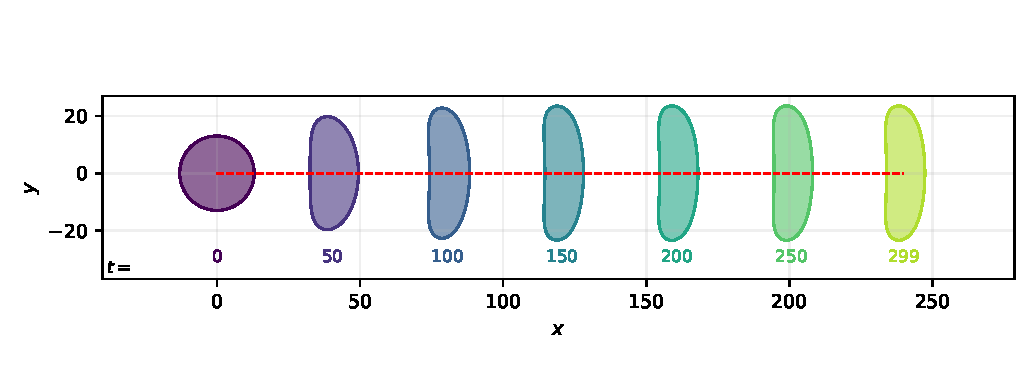
\includegraphics[width=13.4cm,height=2.85cm,keepaspectratio]{figures/fig_v4_montage.pdf}\\[2pt]
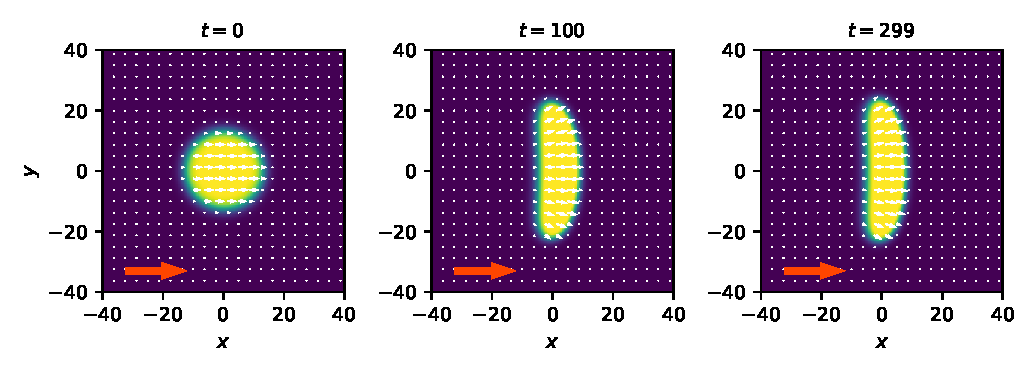
\includegraphics[width=13.4cm,height=2.85cm,keepaspectratio]{figures/fig_v4_snapshots.pdf}\\[2pt]
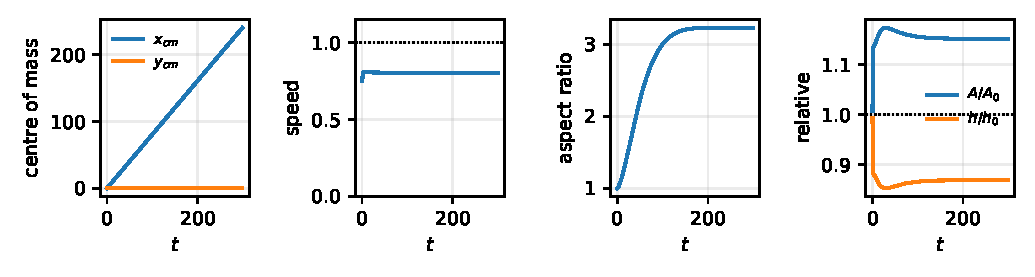
\includegraphics[width=13.4cm,height=2.15cm,keepaspectratio]{figures/fig_v4_diagnostics.pdf}\\[2pt]
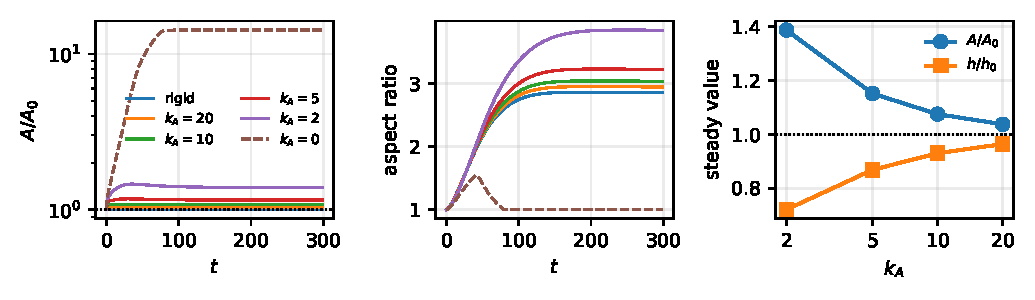
\includegraphics[width=13.4cm,height=2.15cm,keepaspectratio]{figures/fig_v4_area.pdf}
\caption{Version~4 crawling (the main result). (a)~Laboratory-frame
outlines coloured by time; travel $239.9$ at speed $0.801$.
(b)~$\phi$ at $t=0$, $100$, $299$ (red arrow: mean $\mathbf{P}$).
(c)~$x_{\mathrm{cm}}$ (linear), speed ($0.801$), aspect ratio ($\to3.2$),
$A/A_{0}$ and $h/h_{0}$.
(d)~Soft volume: $A/A_{0}(t)$ and aspect ratio for several $k_{A}$;
$k_{A}=0$ inflates $\sim14\times$.}
\label{fig:v4}
\end{figure}

Where Versions~3 and~4 coincide (flow off, rigid area) they agree to
$0.2\%$. Soft volume ($k_{A}=5$) changes speed by $<1\%$ and shape by
$35\%$ (Fig.~\ref{fig:v4}d). Removing the constraint ($k_{A}=0$) inflates
the cell $14$-fold and stops crawling. Cost falls from $2.70$ to
$1.10\,\mathrm{ms}$/step and the stable $dt$ rises from $0.01$ to $0.03$,
about $5\times$ overall.

%%%%%%%%%%%%%%%%%%%%%%%%%%%%%%%%%%%%%%%%%%%%%%%%%%%%%%%%%%%%
\section{Conclusions and future scope}
\label{sec:Conclusion}

\noindent
The four stages are verified. Volume is conserved to machine precision
where it should be. A substrate-confined treadmilling layer produces a
protrusion and a transition at $w_{0}\approx M\varepsilon^{2}/\lambda$
(Fig.~\ref{fig:v2}). The plane model recovers the aster and the
lamellipodial fan (Fig.~\ref{fig:v3}); shape is anchoring-driven
($+2\%$ from flow). Version~4 crawls at speed $0.801$
(Fig.~\ref{fig:v4}), is $\approx5\times$ faster, agrees to $0.2\%$ where
comparable, and is local. Soft volume lets the cell spread and thin;
$k_{A}=0$ is not viable. Next: two cells, collisions, spontaneous
polarity, load-dependent friction~\cite{Leoni:2017}, then collectives.

\section*{Acknowledgements}
The authors thank Prof.\ Sujin B.\ Babu for suggesting the problem and for
guidance on volume conservation and on replacing the Stokes solve.

{\footnotesize
\begin{thebibliography}{99}
\bibitem{Bray:2000}
  D.~Bray, \textit{Cell Movements}, 2nd~ed., Garland (2000).
\bibitem{Verkhovsky:1999}
  A.~B.~Verkhovsky, T.~M.~Svitkina and G.~G.~Borisy, Curr.\ Biol.\ {\bf 9}, 11 (1999).
\bibitem{Keren:2008}
  K.~Keren \textit{et al.}, Nature {\bf 453}, 475 (2008).
\bibitem{Tjhung:2015}
  E.~Tjhung, A.~Tiribocchi, D.~Marenduzzo and M.~E.~Cates, Nat.\ Commun.\ {\bf 6}, 5420 (2015).
\bibitem{Leoni:2017}
  M.~Leoni and P.~Sens, Phys.\ Rev.\ Lett.\ {\bf 118}, 228101 (2017).
\bibitem{Ziebert:2013}
  F.~Ziebert and I.~S.~Aranson, PLoS ONE {\bf 8}, e64511 (2013).
\bibitem{Rubinstein:1992}
  J.~Rubinstein and P.~Sternberg, IMA J.\ Appl.\ Math.\ {\bf 48}, 249 (1992).
\bibitem{Yam:2007}
  P.~T.~Yam \textit{et al.}, J.\ Cell Biol.\ {\bf 178}, 1207 (2007).
\end{thebibliography}
}
\end{document}
